\chapter{Background} \label{ch:background}

The advent of video microscopy brought the dynamic nature of the organelle environment into focus in the 1980s. Soon after, Ron Vale and colleagues discovered the identity of one of the proteins responsible for the observed transport, kinesin. In the more than 30 years since this discovery, we have learned a great deal about each of the components of the transport system from a combination of careful in vivo and in vitro experimental work, as well as enlightening modeling efforts.

\section{Microtubules}

Eukaryotic cells possess a microtubule (MT) network, composed of hundreds of individual MT filaments. Recently, super-resolution microscopy has allowed imaging and mapping of the entire MT network with a single MT resolution \cite{Zhang2016}, as shown in figure \ref{fig:MTcytoskeleton}. Individual MTs are dynamic, assembling and disassembling stochastically \cite{Howard2003}. This allows the MT network to be reorganized as cells move and change shape, as well as in response to external cues \cite{Herms2015,Zhu2015,Zhang2016}. 

\begin{figure}
\centering
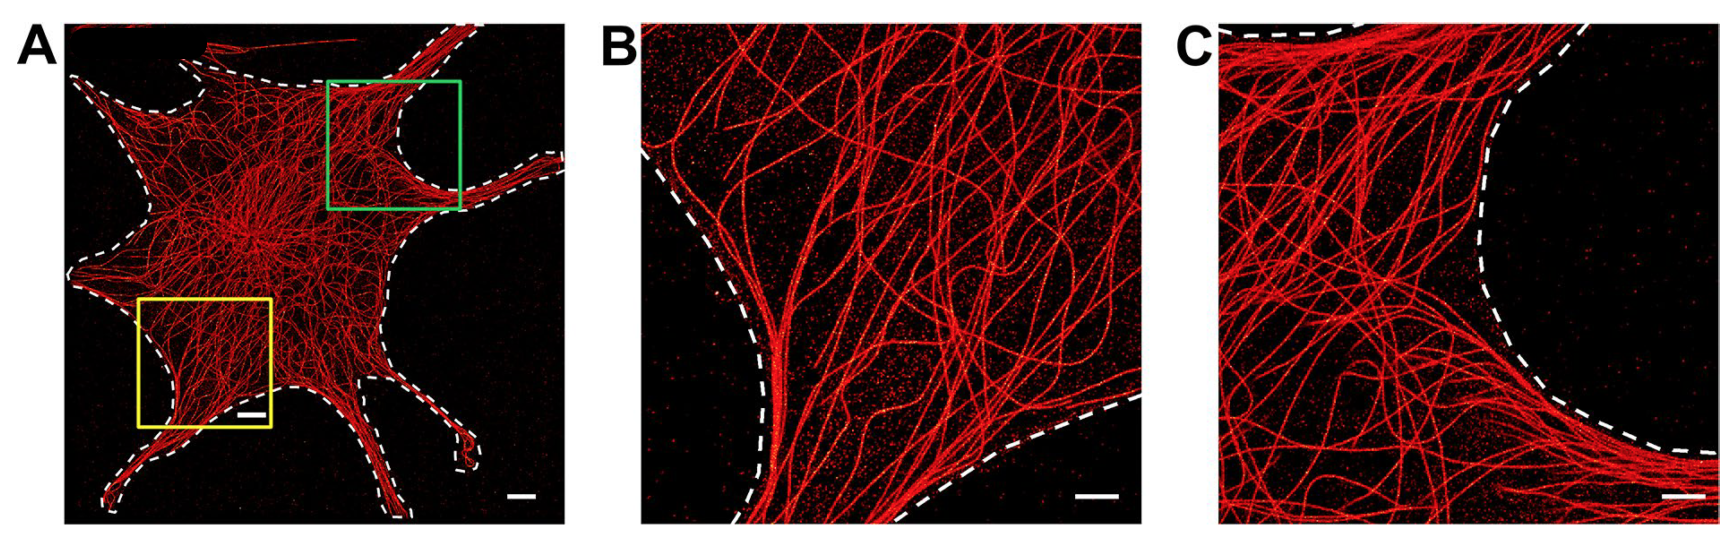
\includegraphics[scale=.5]{background/MTcytoskeleton}
\caption[Super-resolution image of a MT network]{An example of a super-resolution image of an entire MT network of a cell (A), adapted from \cite{Zhang2016}. Single MTs are identifiable from fluorescence labelling in red. Region in yellow box magnified in (B), region in green box magnified in (C). Scale bars are \SI{5}{\micro\meter} in panel A and \SI{2}{\micro\meter} in panels B and C.}
\label{fig:MTcytoskeleton}
\end{figure}

The MT network serves many functions in the cell. Most importantly for the work in this document, MTs serve as the ``roads'' along which cargos are transported. In addition to this role, MTs are a component of the of the cytoskeleton, which gives cells shape and structure. Furthermore, MTs bear the forces exerted to divide chromosomes between the daughter cells in cell division. 

The structure of MTs allow them to perform these functions. MTs are tubular, consisting of a number of linear protofilaments assembled into a ring \cite{Grimstone1966} as shown in figure \ref{fig:MTstructure}. MTs commonly have 13 or 14 protofilaments \cite{Pierson1978}, but that number can vary from fewer than 9 to more than 15 depending on organism and cell type\cite{Davis1983}. Each protofilament is a repeating polymer of dimers of $\alpha$ and $\beta$ tubulin subunits. This repeating structure makes it possible for kinesin and dynein to move processivley along the MT outer surface. MT structures can have defects, and it has been shown these defects can influence transport \cite{Liang2016}.

\begin{figure}
\floatbox[{\capbeside\thisfloatsetup{capbesideposition={right,top}}}]{figure}[\FBwidth]
{\caption[Microtubule Structure]{The structure of a microtubule is shown, demonstrating the tubular structure composed of linear protofilaments made up of repeating dimers of $\alpha$ and $\beta$ subunits. Illustration \href{https://en.wikipedia.org/wiki/Microtubule\#/media/File:Microtubule_structure.png}{``Structure of a microtubule''} by \href{https://commons.wikimedia.org/wiki/User:Splette}{Thomas Splettstoesser} is licensed under \href{https://creativecommons.org/licenses/by-sa/4.0/}{CC BY-SA 4.0.}}
\label{fig:MTstructure}}
{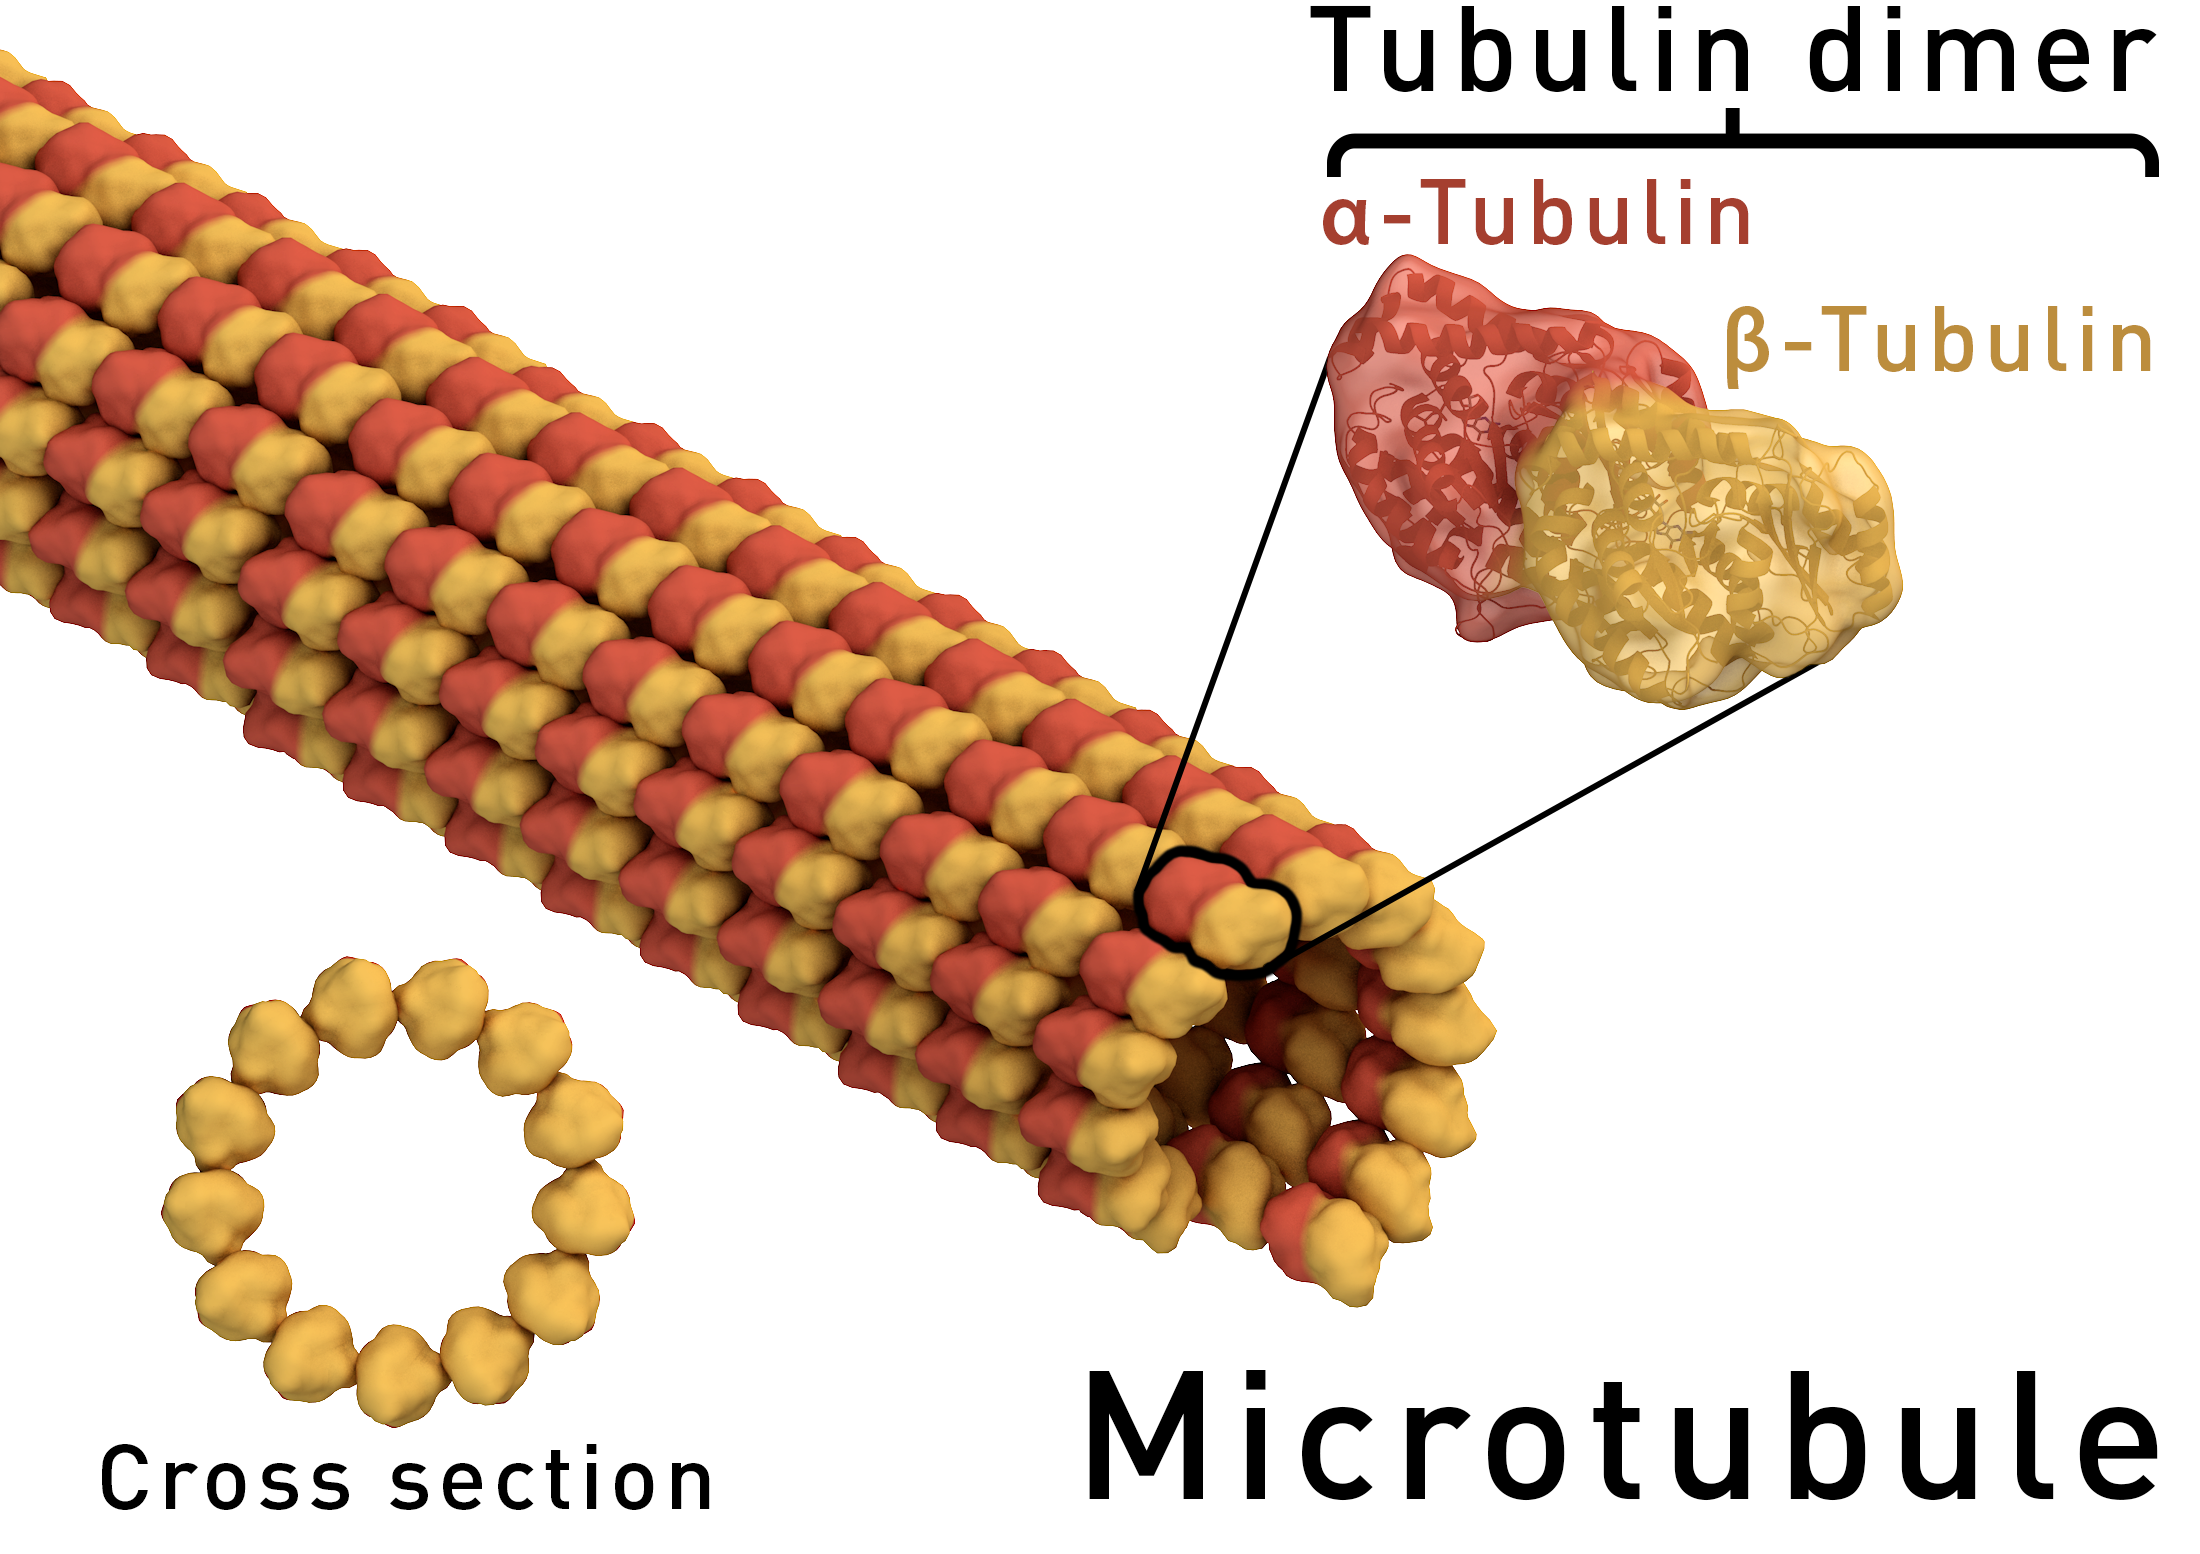
\includegraphics[scale=.1]{background/Microtubule_structure}}
\end{figure}

The tubular structure makes MTs rigid compared to other cellular filaments such as actin, with persistence lengths near \SI{1}{\milli\meter}, many times the size of an entire cell. Rigidity can vary with MT length and repeated bending \cite{Schaedel2015}.

\subsection{Microtubule Associated Proteins}

In cells, MTs are decorated with a variety of proteins deemed microtubule associated proteins (MAPs). MAPs have been found to play roles in stabilizing and destabilizing MTs, as well as aiding in localizing and organizing MTs \cite{Mandelkow1995}. The MAP tau is associated with a variety of neurodegenerative diseases deemed ``tauopathies", including Alzheimer's disease and chronic traumatic encephalopathy \cite{Kovacs2015}. Since tau overexpression has been shown to hinder transport in neurons \cite{Stamer2002}, as well as to differentially affect the ability of kinesin and dynein to transport cargo in vitro \cite{Vershinin2007,Vershinin2008,Dixit2008}, malfunctions in cargo transport have been implicated in the cause of neurodegeneration in tauopaties. The heterogenious distribution of tau in neurons \cite{Black1996,Kempf1996} supports a possible role for tau in localized cargo delivery.

\subsection{Microtubule Post-translational Modifications}

Tubulin possess several sites known to undergo different post-translatinoal modifications (PTMs), many of which are reversible \cite{Garnham2012}. These sites are predominantly located in the C-terminal tail region, located on the outer MT surface as shown in figure \ref{fig:PTMs}. PTMs are distributed heterogeneously on the MT network \cite{Garnham2012}, with specific subsets of modified MTs implicated in transport of specific cargos \cite{Herms2015}.

A survey of the impact of various PTMs on motor behavior \cite{Sirajuddin2014} showed that a single PTM can impact one or more motor properties, as well as impacting different motors in different ways. Furthermore, different PTMs have different impacts on a single motor. The richness of this behavior lends credence to the `tubulin-code' hypothesis, which predicts that combinations of tubulin isotypes, PTMs and MAPs encode directions for the localization and activity of cargos and other proteins. Modeling shows that even weak localization of PTMs may be able to direct strong cargo localization \cite{Iniguez2016}.

\begin{figure}
\floatbox[{\capbeside\thisfloatsetup{capbesideposition={right,top}}}]{figure}[\FBwidth]
{\caption[Microtubule Post-translational Modification Sites]{Microtubules undergo post-translational modifications at a variety of sites, mostly in the C-terminal tail region located on the outside MT surface. Figure from \cite{Garnham2012}.}
\label{fig:PTMs}}
{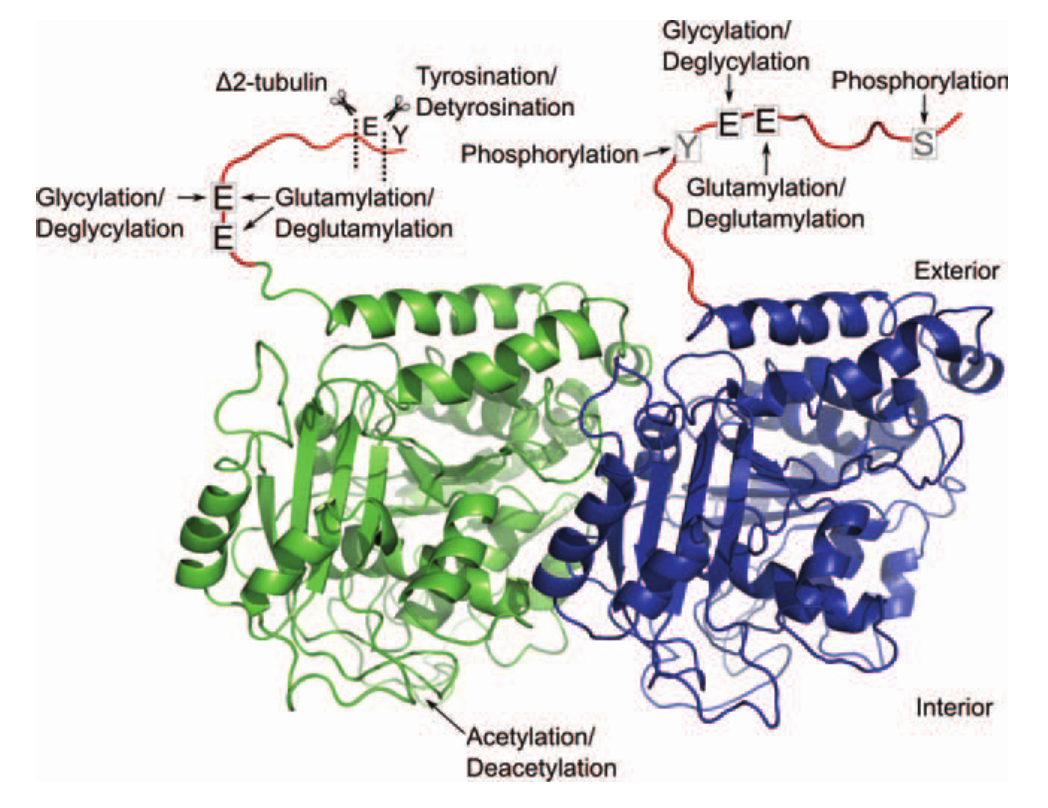
\includegraphics[scale=.6]{background/PTMs}}
\end{figure}

\section{Molecular Motors}

Molecular motors are a class of enzymes (specifically ATPases), which convert the chemical energy bound up in ATP into mechanical work. There are three classes of molecular motors involved in cargo transport: kinesin superfamiliy motors and cytoplasmic dynein which walk along microtubules, and myosin superfamily motors which walk along actin. Here we'll focus on the former two motors.

\subsection{Kinesin} \label{sec:kinesin}

The defining feature of a kinesin is the kinesin motor domain, which binds to MTs and is responsible for ATP hydrolysis \cite{Verhey2011}. Hundreds of genes which include the kinesin motor domain have been identified across a variety of different organisms; together these genes make up the kinesin superfamily. This superfamily has been divided into 14 families based on function and sequence similarity \cite{Lawrence2004}. In mice, there are 45 individual kinesins which perform a variety of tasks in the cell, from transporting cargo to MT depolymerization \cite{Hirokawa2009}. The motors which have established roles in transport are the members of the kinesin-1 (KIF5), kinesin-2 (KIF3) and kinesin-3 (KIF1) families \cite{Verhey2011}. Kinesin-1 is the most well studied family, also called conventional kinesin. It is a heterotetramer of a kinesin heavy chain homodimer and two kinesin light chain subunits, as shown in figure \ref{fig:kinesin_types}. Kinesin-2 can exist either as a homodimer or heterodimer of different motor domain containing subunits, with each form associated with different motility properties. However, the motility mechanism of kinesin-2 is similar to kinesin-1 \cite{Andreasson2015}. Kinesin-2 motors also tend to switch protofilaments while walking, resulting in a spiral path around the MT \cite{Brunnbauer2012}, where kinesin-1 motors walk a straight line \cite{Ray1993}. Kinesin-3 motors exhibit limited motility as a monomer, but likely work as dimers in vivo, similar to kinesin-1 and kinesin-2 motors \cite{Siddiqui2017}. We will focus on kinesin-1 for the rest of this section and will refer to it simply as kinesin.

\begin{figure}
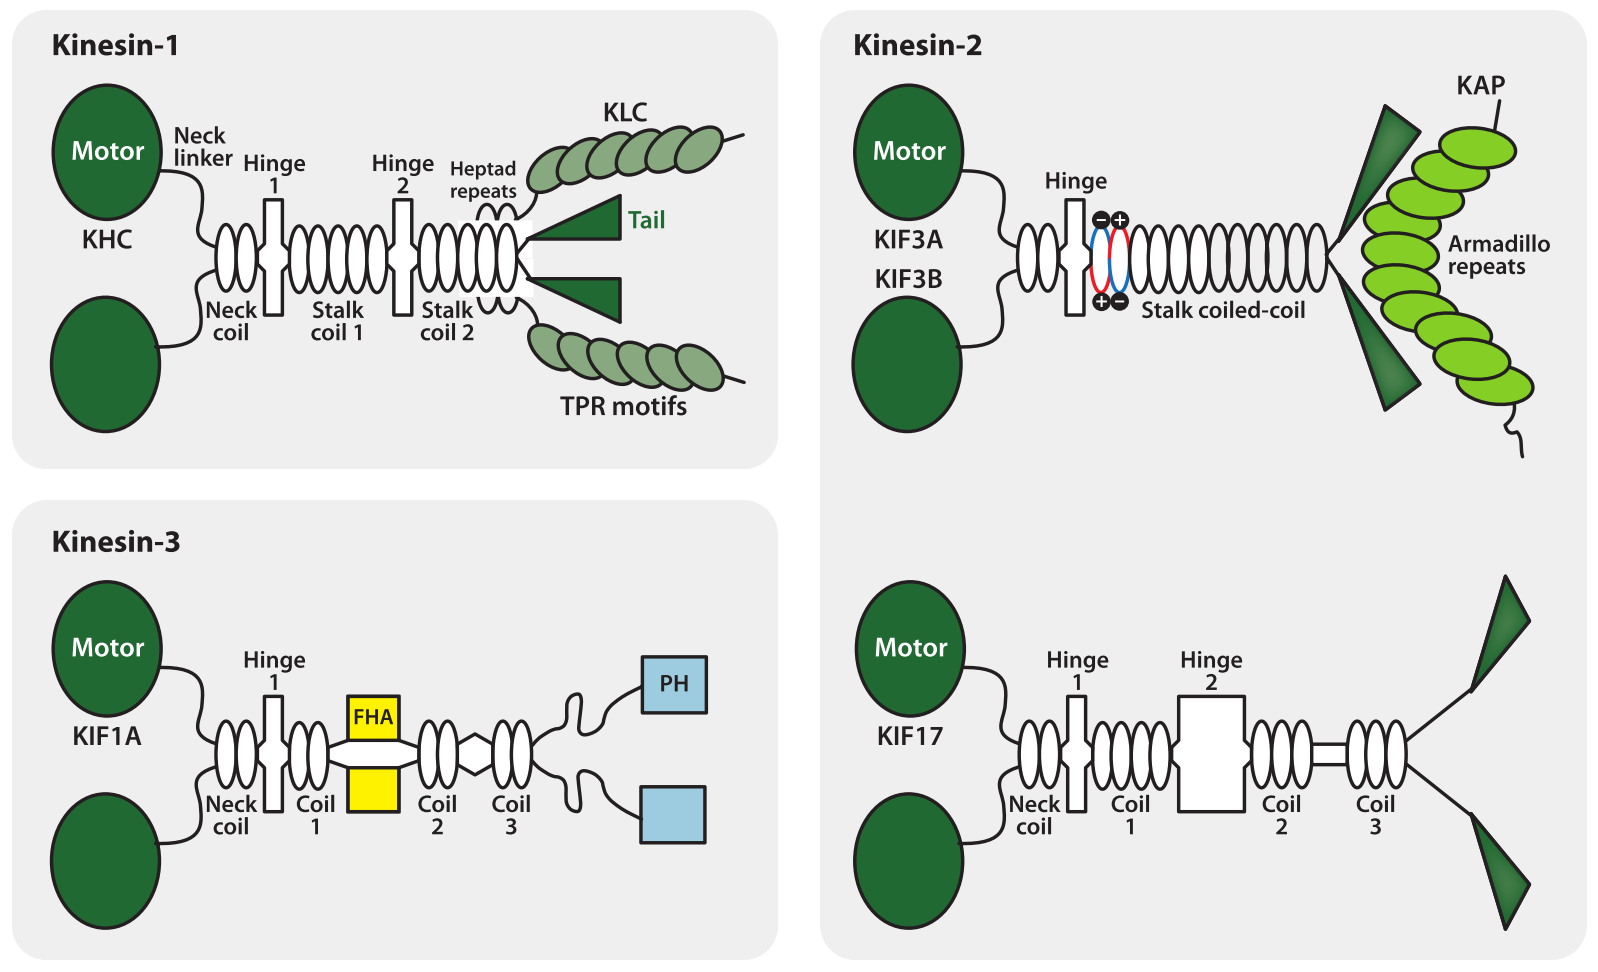
\includegraphics[width=\textwidth]{background/kinesin_types}
\caption[Composition of transport kinesins]{Subunit composition of transport kinesins. Kinesin-1 or conventional kinesin is the most well studied motor family. Kinesin-2 and kinesin-3 are less studied, but also known to transport cargos in cells. Kinesin motor domins are the defining feature of the kinesin superfamily and are shown as green ovals. Kinesin motors domains bind to the MT, which the other end of the motors bind cargos or linkers. Abbreviations: FHA, forkhead associated; KAP, kinesin-associated protein; KHC, kinesin heavy chain; KIF, kinesin family; KLC, kinesin light chain; PH, pleckstrin homology; TPR, tetratricopeptide repeat. Figure from \cite{Verhey2011}.}
\label{fig:kinesin_types}
\end{figure}

Kinesin motors step processively along MT tracks in a hand-over-hand fashion, with each motor domain taking \SI{16}{\nano\meter} steps \cite{Yildiz2004} that move the center of mass of the motor forward by \SI{8}{\nano\meter} \cite{Svoboda1993}. When unloaded, kinesin steps quickly, moving about \SI{1}{\micro\meter\per\second}. Times between steps are exponentially distributed \cite{Carter2005}. Velocity reduces under increasing resistive load until stall, which occurs at $\approx$ \SI{6}{\pico\newton}. The nature of this decrease has been found to be superlinear in some studies \cite{Kunwar2010,Visscher1999,Fallesen2011,Rai2013}, while others find more linear behavior \cite{Svoboda1994,Andreasson2015a}.

Kinesin unbinds from the microtubule at a rate that also depends on the load experienced by the motor. Several reports agree that unbinding rate increases with load exponentially up to the stall force, but disagree about behavior above stall. One study claims unbinding rate increases only quickly above stall \cite{Kunwar2011}, while another claims unbinding rate continues to increase exponentially \cite{Andreasson2015a}. The unbinding rate has been found to depend on the directionality of the load applied. Hindering loads result in the aforementioned behavior, while assisting loads result in an increased unbinding rate \cite{Milic2014,Andreasson2015a}. Sideways loads result in slightly asymmetrical unbinding behavior \cite{Block2003}.

It has been found that the kinesin stalk is stiff in tension \cite{Kojima1997} and also resists compression to a lesser degree \cite{Jeney2004}. It has little resistance to torsion \cite{Hunt1993,Gutierrez-Medina2009}.

\subsection{Dynein}

Like kinesin, cytoplasmic dynein-1 is a homodimeric motor which processively steps along MTs. However, unlike kinesin, there is only one dynein that transports cargos in the cytoplasm \cite{Bhabha2016}. Also unlike kinesin, the two dynein heads step largely independently of each other \cite{DeWitt2012}. Furthermore, dynein step sizes are variable and often include sideways and backward steps \cite{Bhabha2016}. Purified mammalian dynein motors are quite weak in vitro, exerting only \SI{1}{\pico\newton} of force \cite{Mallik2004} compared with kinesin's \SI{6}{\pico\newton}.

Several sets of proteins are known to regulate dynein force production. Lis1 and NudE work together to put dynein into a persistent force producing state in vitro \cite{McKenney2010}. These proteins are also necessary for the recently discovered force adaptation under load displayed by lipid droplets in vivo \cite{Reddy2016}. Dynactin seems to be involved in almost every task carried out by dynein \cite{Cianfrocco2015}. When paired with one of the adaptor proteins BicD2, Rab11-FIP3, Spindly, or hook, it is capable of dramatically increasing dynein's processivity \cite{McKenney2014}. Furthermore, dynein-dynactin-BicD2 complexes exert much higher forces in vitro, stalling at \SI{5}{\pico\newton}, comparable to kinesin \cite{Belyy2016}.

\begin{figure}
\floatbox[{\capbeside\thisfloatsetup{capbesideposition={right,top}}}]{figure}[\FBwidth]
{\caption[Dynein and its regulators]{A cartoon of dynein, showing its domains. Included in the inset are proteins known in regulate dynein function. Figure from \cite{Kardon2009}.
\label{fig:dynein}}}
{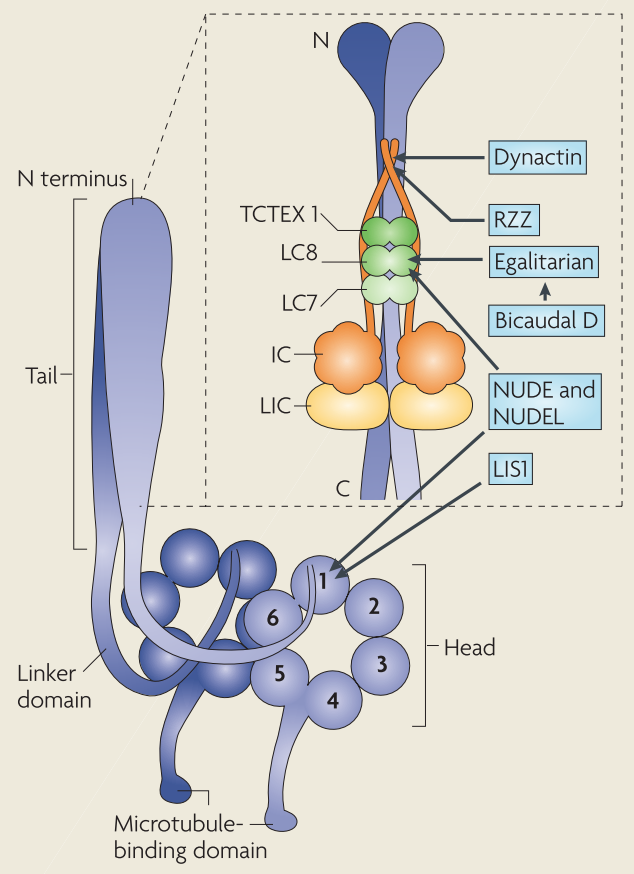
\includegraphics[scale=.5]{background/dynein_interactors}}
\end{figure}

\section{Cargos}

A wide variety of organelle cargos such as lipid droplets, mitochondria, melanosomes, peroxisomes, pigment granules, endosomes, secretory vesicles, RNA granules, and virions are transported bi-directionally by molecular motors \cite{Hancock2014,Gross2004}. Long distance cargo transport is also particularly important in neurons. Cargos such as dense core vesicles carrying neuropeptide and synaptic vesicles carrying neurotransmitter must be transported down the length of axons, often millimeters to centimeters long, and delivered at presynapses \cite{Maeder2014}. These observations lead to a picture of cargo transport where bidirectional motion is controlled to correctly localize cargos, as shown in figure \ref{fig:cargo_delivery}.

\begin{figure}
\centering
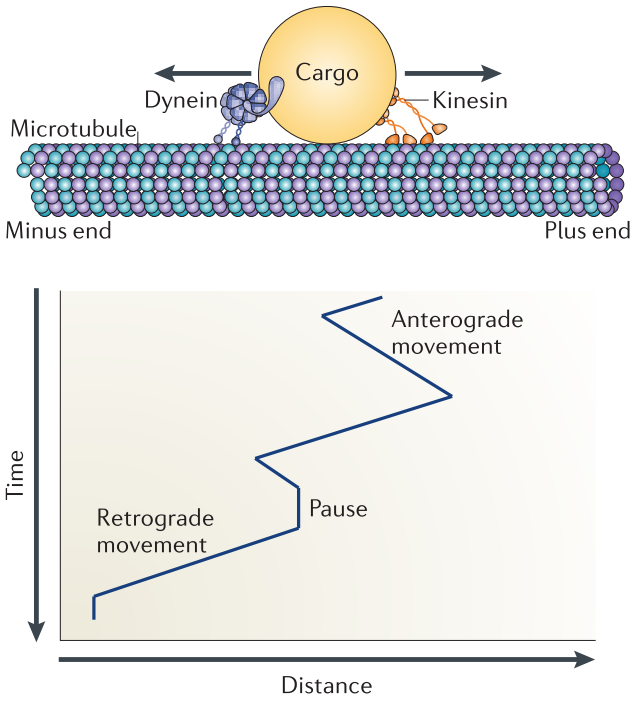
\includegraphics[width=.45 \textwidth]{background/bidirectional_motion}
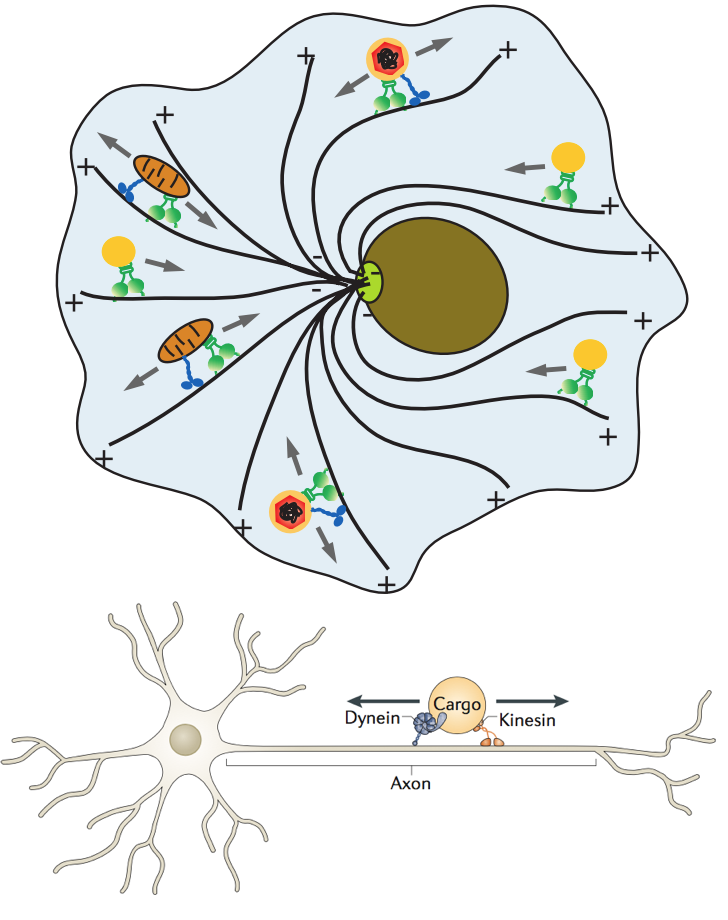
\includegraphics[width=.45 \textwidth]{background/cargo_delivery}
\caption[Bidirectional motion and cargo delivery]{A variety of cargos have been shown to move bidirectionally on MTs in cells, as shown on the left. By biasing this bidirectional motion, the cell may be able to deliver cargos to specific locations in neurons and other cell types, as shown on the right. Figures on left and bottom right from \cite{Hancock2014}. Figure on top right from \cite{Gross2004}.}
\label{fig:cargo_delivery}
\end{figure}

\subsection{Lipid Droplets}

Lipid droplets (LDs) contain the cell's store of neutral lipids. These lipids can be used to create new membranes, or broken down to be used in metabolism when glucose supplies are lacking. LDs consist of a core of neutral lipids, surrounded by a single layered phospholipid membrane. \cite{Welte2015}.

The lipid core gives the LD a contrasting index of refraction compared to the surrounding cytoplasm. This makes the LD an ideal target for both DIC microscopy and optical trapping \cite{Reddy2016}. The importance of transport to LD biology is highlighted in a recent study that showed LDs move from the near the membrane (where the lipid supplies are putatively being used to make new membrane) into contact with mitochondria when the cell is starved of glucose \cite{Herms2015}.

\section{Previous models of cargo transport}

An early model of multiple motor cargo transport posed the problem as a Markov chain, with state transitions representing binding and unbinding of the motors \cite{Klumpp2005}. It was shown this model was able to reproduce a variety of the behaviors observed in vivo \cite{Muller2008}. Despite its success, it was difficult to interpret how experimentally observed parameters translated to model parameters, including how forces are shared between multiple motors and the stochastic nature of motor stepping.

A subsequent model represented motors as two points, with forces in each generated by the stretch in spring-like motor stalks \cite{Kunwar2008}. While only one dimensional spatially, this model was able to elucidate many details of how multiple motors might work together \cite{Kunwar2010}. In a surprising negative result, the Gross lab showed that neither model was able to match the behavior of cargos in vivo when supplied with realistic single motor behavior \cite{Kunwar2011}.

Three dimensional models of cargo transport have also since been constructed \cite{Korn2009,Erickson2011,Lombardo2017}. They have been used to investigate the impact of how motors are arranged on a cargo \cite{Erickson2011} and cargo switching between filiments \cite{Erickson2013}. Recently, a model of cargo transport included the ability for motors to diffuse in the cargo membrane in 3D \cite{Lombardo2017}.